\subsection{Jet Trigger Efficiency}
\label{sec:jet_trigger_efficiency}

Jet trigger efficiencies were evaluated using runs from the ana509 Good Run List where the Jet10 (trig22) was not prescaled, comprising 1482 runs after excluding 50 runs where trig22 was turned off or prescaled. 
The analysis focuses on the Jet10 triggers (trigger definitions are included in list below) and examines the effects of vertex selections, beam crossing angle, jet background rejection cuts, trigger logic mappings, and detector-related effects.

Trigger efficiencies are measured as a function of offline reconstructed jet transverse energy using minimum bias coincidence (MB) triggers as the reference. 
Unless otherwise noted, scaled trigger bits are used, with no scaledowns applied to the jet triggers (trig22, trig18 and trig34). 
The baseline efficiency definition is:
\begin{equation}
\epsilon_{\mathrm{Jet10}} =
\frac{N(\mathrm{Jet10} \cap \mathrm{MB})}{N(\mathrm{MB})}.
\end{equation}

\subsubsection{0~mrad vs.\ 1.5~mrad Running}

Various selections of Jet10 triggers and MB triggers are studied to determine the efficiency of the Jet10 trigger. The trigger definitions are as follows:
\begin{itemize}
    \item Jet10 (trig22)
    \item Jet10 + MB (trig18)
    \item Jet10 + MB + $|z_{\mathrm{vtx}}| < 10$~cm (trig34)
    \item MB (trig10)
    \item MB + $|z_{\mathrm{vtx}}| < 10$~cm (trig12)
\end{itemize}
These multiple selections of Jet10 triggers and MB triggers are studied since, on the whole, trig10 and trig18 were turned on and trig12 and trig34 were turned off in the 0 mrad running.
While for the majority of the runs in the 1.5 mrad dataset, trig12 and trig34 were turned on and trig10 and trig18 were turned off.
Therefore, it is important to study the efficiency of the Jet10 trigger (trig22) with the two different MB reference triggers (trig10 and trig12) and in both run ranges (0 mrad and 1.5 mrad running) since the analysis uses jet triggers across both run ranges.

The jet trigger efficinecies are determined using the leading uncalibrated jet transverse momentum from minimum bias and minimum bias + jet triggered events.
These uncalibrated leading jet spectra are shown in Figure~\ref{fig:mb_jet_spectra}.
Figure~\ref{fig:mb_jet_spectra} left (right) shows the comparison of the MB and MB + jet trigger events from the 0mrad (1.5mrad) running.

\begin{figure}
    \centering
    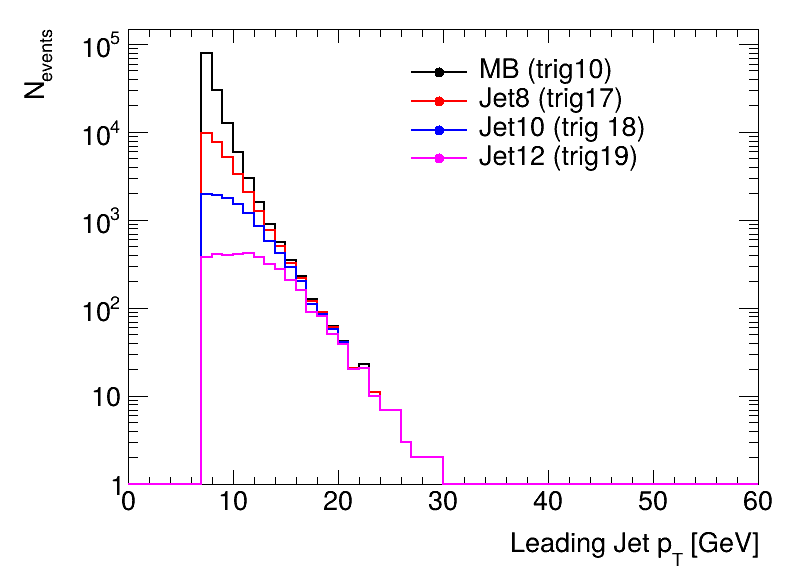
\includegraphics[width=0.48\linewidth]{Figures/trigger_efficiency/0mrad_all_jet_events.png}
    
\includegraphics[width=0.48\linewidth]{{Figures/trigger_efficiency/1.5mrad_all_jet_events}.png}
    \caption{Comparison of the MB (black) and MB + jet trigger events for Jet8 (red), Jet10 (blue) and Jet12 (magneta). Comparison is shown for both the 0 mrad (left) and 1.5 mrad (right) running.}
    \label{fig:mb_jet_spectra}
\end{figure}

The first test of the jet trigger efficiency was to compare the efficiency of the Jet10 trigger (trig22) extracted using the two different possible MB reference triggers (trig10 and trig12). 
A comparison of the efficiency of the Jet10 trigger (trig22) with the two different MB reference triggers (trig10 and trig12) is shown in Figure~\ref{fig:trig22_reference_trig_comparison}.
Here the efficiency for trig18(22)/trig10 is determined only for runs where trig18(22) was not prescaled and trig10 was turned on.
Similarly, the efficiency for trig34(22)/trig12 is determined only for runs where trig34(22) was not prescaled and trig12 was turned on.
Good agreement is observed between the trig18(22)/trig10 and trig34(22)/trig12 efficiency curves in both Figure~\ref{fig:trig22_reference_trig_comparison} left and right which correspond to 0mrad and 1.5mrad running respectively.
Therefore, the overall efficiency of the Jet10 trigger (trig22) determined from these two different MB reference triggers (trig10 and trig12) is consistent.

\begin{figure} 
    \centering
    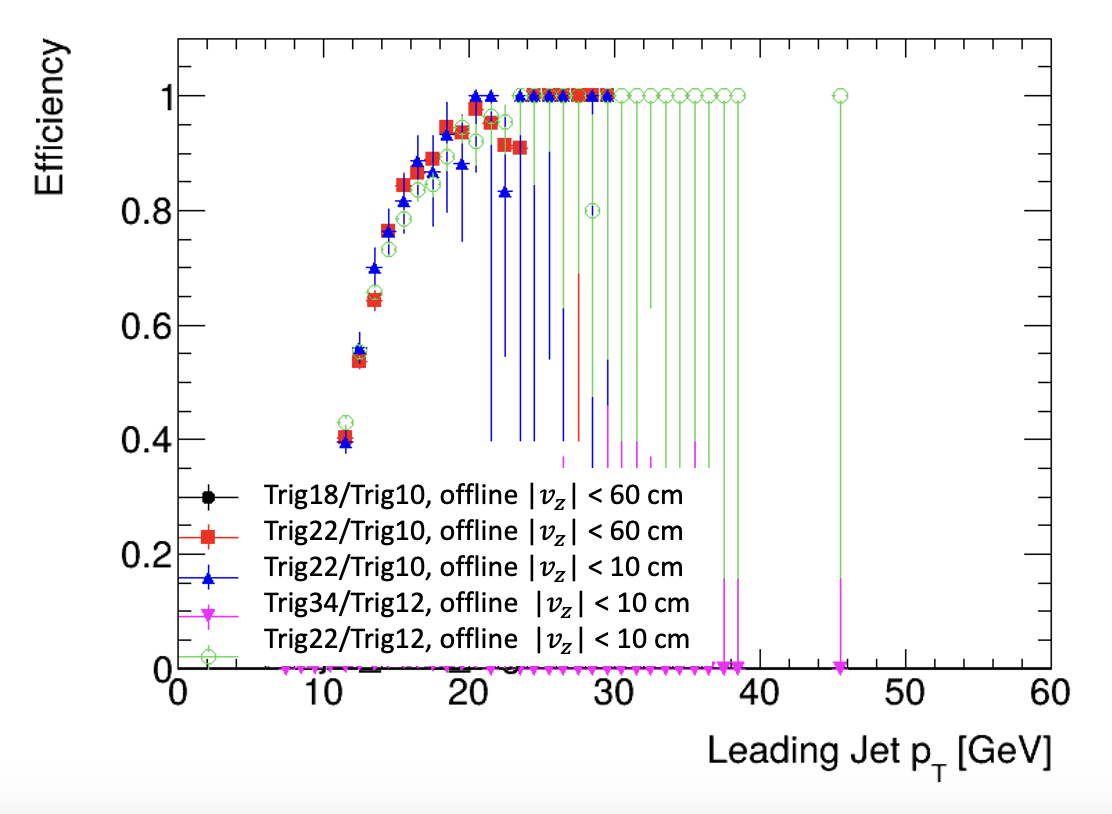
\includegraphics[width=0.48\linewidth]{Figures/trigger_efficiency/0mrad_efficiency_comparison.png}
    
\includegraphics[width=0.48\linewidth]{{Figures/trigger_efficiency/1.5mrad_efficiency_comparison}.png}
    \caption{Comparison of the efficiency of the Jet10 trigger for different MB reference triggers in both the 0 mrad (left) and 1.5 mrad (right) running.}
    \label{fig:trig22_reference_trig_comparison}
\end{figure}

Following this first comparison of the MB reference trigger influence on the Jet10 trigger efficiency, a comparison of the efficiency of the Jet10 trigger (trig22) in both the 0 mrad and 1.5 mrad running is shown in Figure~\ref{fig:trig22_run_range_comparison}.
Here, the efficiency for trig22/trig10 is determined only for runs where trig22 was not prescaled and trig10 was turned on.
Similarly, the efficiency for trig22/trig12 is determined only for runs where trig22 was not prescaled and trig12 was turned on.
Note that comparisons here are made between the trig22/trig10 efficiency for 0 mrad and trig22/trig12 efficiency for 1.5 mrad in order to use the largest statistics possible for each run range and since the previous study showed good agreement between the efficinecy from the two different MB reference triggers when using the same run ranges.
A 20\% difference is observed between the 0 mrad trig22/trig10 efficiency (open red) and 1.5 mrad trig22/trig12 efficiency (open orange).

\begin{figure}
    \centering
    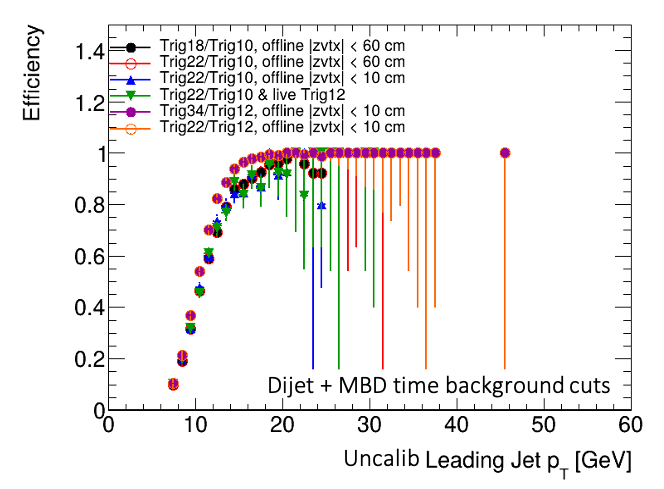
\includegraphics[width=0.48\linewidth]{Figures/trigger_efficiency/dijet_mbdtime_jet_trig_comp.png}
    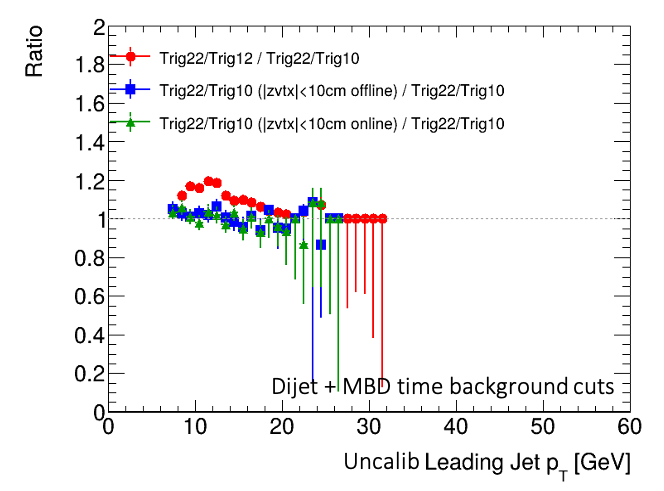
\includegraphics[width=0.48\linewidth]{Figures/trigger_efficiency/dijet_mbdtime_jet_trig_ratio.png}
    \caption{Comparison (left) and ratio (right) of the efficiency of the Jet10 trigger for different run ranges (0 mrad trig22/trig10 and 1.5 mrad trig22/trig12).}
    \label{fig:trig22_run_range_comparison}
\end{figure}

Investigations into the source of this difference were undertaken and are also included in Figure~\ref{fig:trig22_run_range_comparison}.
These studies include applying an offline vertex cut of $|z_{\mathrm{vtx}}| < 10$~cm to the 0 mrad trig22/trig10 efficiency (solid blue) as well as requiring an online vertex cut of $|z_{\mathrm{vtx}}| < 10$~cm (require live trigger bit trig12) on the 0 mrad trig22/trig10 efficiency (solid green).
The online vertex cut was applied here by requiring the live trigger bit trig12 to be on, 
which ammended the efficiency calculation to $\epsilon = \frac{\mathrm{trig22}_{\mathrm{live}} + \mathrm{trig12}_{\mathrm{live}} + \mathrm{trig10}_{\mathrm{scaled}}}{\mathrm{trig12}_{\mathrm{live}} + \mathrm{trig10}_{\mathrm{scaled}}}.$

The resulting efficiencies from including both the offline and online vertex cuts do not show any discrepancy from the original 0 mrad trig22/trig10 efficiency (open red).
Therefore, these vertex cuts do not seem to be the source of the difference between the 0 mrad trig22/trig10 efficinecy and the 1.5 mrad trig22/trig12 efficiency.
However, these differences in the efficiency can be caused by other effects such as changes in the calorimeter response and calibration across the full Run 2024 dataset.
Therefore, further investigations into the run by run stability of the Jet10 trigger efficiency and a run range dependent efficiency are undertaken in the section on run by run dependence below and implemented in into the final efficiencies for the analysis.

\subsubsection{Jet Background Rejection Cuts}

The influence of jet background rejection cuts was studied by applying energy fraction cuts, dijet cuts, jet-MBD timing cuts, and a jet multiplicity requirement of $N_{\mathrm{jet}} \leq 9$. 
These cuts are described in more detail in the jet background section of the analysis.

A breakdown of the Jet10 trigger efficiency for the 0 mrad and 1.5 mrad datasets for these individual background cuts is shown in Figure ~\ref{fig:jet_bkg_cuts_comparison}.
Here, the energy fraction cuts create the largest difference in efficinecy between the 0 mrad and 1.5 mrad datasets, which seems reasonable since the jet trigger is configured based on fractions of energy in each calorimeter layer. 
The dijet and and dijet + MBD timing cuts have a comparatively smaller effect on the trigger efficiency difference between the 0 mrad and 1.5 mrad datasets.

\begin{figure}
    \centering
    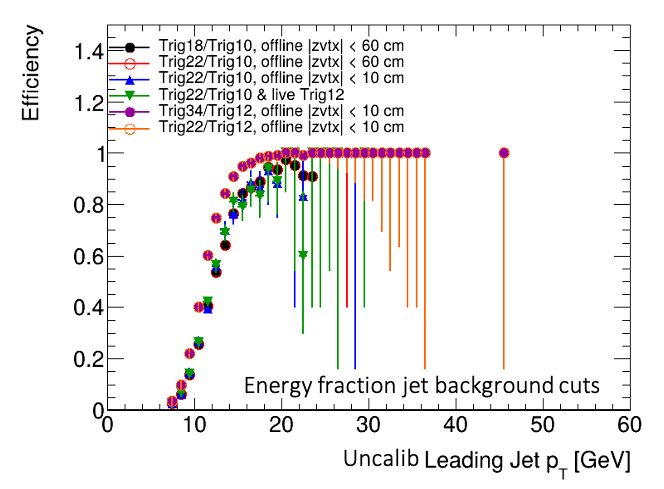
\includegraphics[width=0.48\linewidth]{Figures/trigger_efficiency/efrac_jet_trig_comp.png}
    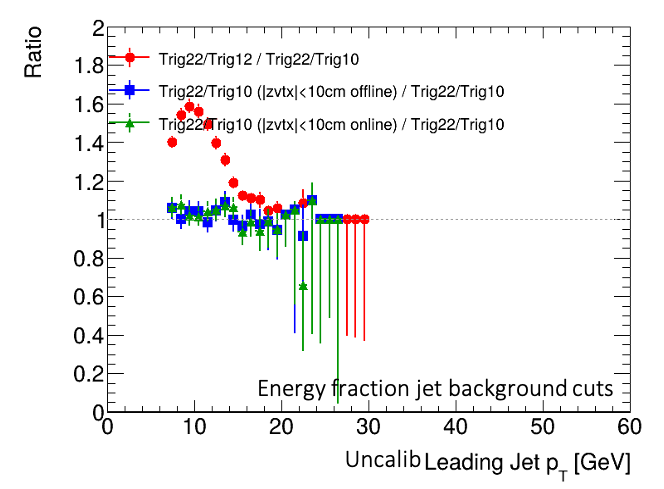
\includegraphics[width=0.48\linewidth]{Figures/trigger_efficiency/efrac_jet_trig_ratio.png}
    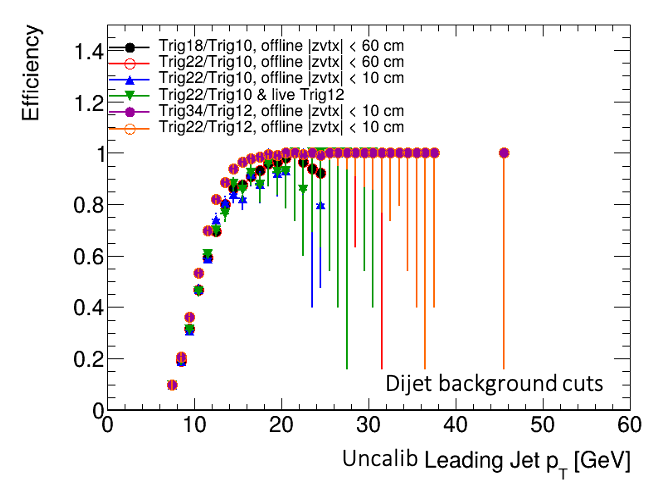
\includegraphics[width=0.48\linewidth]{Figures/trigger_efficiency/dijet_jet_trig_comp.png}
    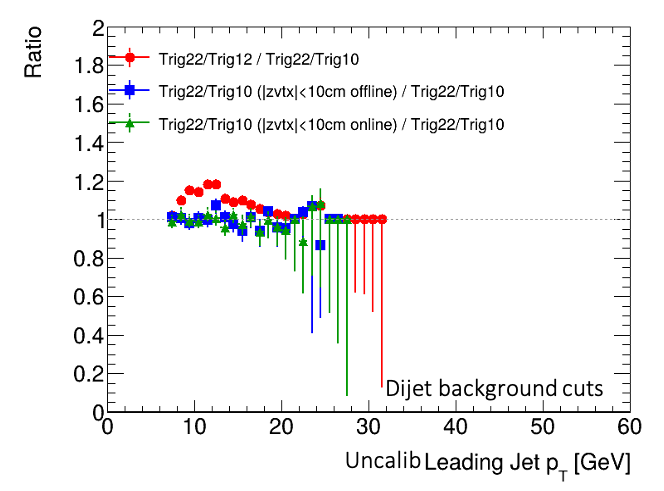
\includegraphics[width=0.48\linewidth]{Figures/trigger_efficiency/dijet_jet_trig_ratio.png}
    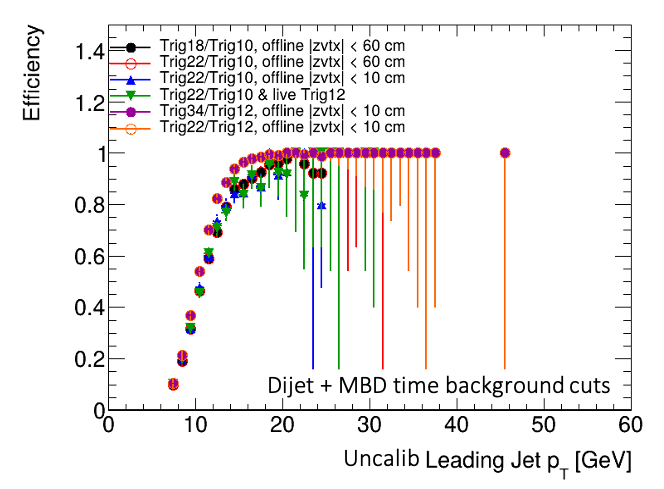
\includegraphics[width=0.48\linewidth]{Figures/trigger_efficiency/dijet_mbdtime_jet_trig_comp.png}
    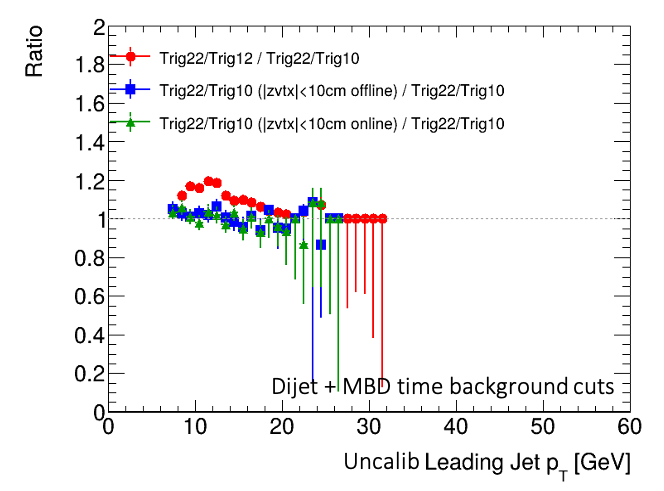
\includegraphics[width=0.48\linewidth]{Figures/trigger_efficiency/dijet_mbdtime_jet_trig_ratio.png}
    \caption{Comparison of the efficiency (left) and ratio (right) of the Jet10 trigger for different jet background cut selections. Energy fraction background cuts are shown in the top plots, dijet background cuts in the middle plots and dijet + MBD timing cuts in the bottom plots.}
    \label{fig:jet_bkg_cuts_comparison}
\end{figure}

%\subsubsection{Detector Mapping Effects}

%Due to a small mapping error in one quadrant of the HCal cotribution to the jet triggers, an investigation into the effect of this mismapping was undertaken.
%The calorimeter barrel is divided into 4 quadrants, with Quadrant 0 corresponding to $0 \leq \phi < \pi/2$, Quadrant 1 corresponding to $\pi/2 \leq \phi < \pi$, Quadrant 3 corresponding to $\pi \leq \phi < 3\pi/2$, and Quadrant 1 corresponding to $3\pi/2 \leq \phi < 2\pi$.
%Quadrant 2 is the quadrant with the known mismapping in the HCal trigger.
%A study of the effect of this mismapping on the Jet10 trigger efficiency is shown in Figure~\ref{fig:quad2_small_effect}.

%\begin{figure}
%    \centering
%    
\includegraphics[width=0.48\linewidth]{{Figures/trigger_efficiency/1.5mrad_quadrant_comparison_leadjet_zcut_jet8}.png}
%    
\includegraphics[width=0.48\linewidth]{{Figures/trigger_efficiency/1.5mrad_quadrant_ratio_leadjet_zcut_jet8}.png}
%    
\includegraphics[width=0.48\linewidth]{{Figures/trigger_efficiency/1.5mrad_quadrant_comparison_leadjet_zcut_jet10}.png}
%    
\includegraphics[width=0.48\linewidth]{{Figures/trigger_efficiency/1.5mrad_quadrant_ratio_leadjet_zcut_jet10}.png}
%    
\includegraphics[width=0.48\linewidth]{{Figures/trigger_efficiency/1.5mrad_quadrant_comparison_leadjet_zcut_jet12}.png}
%    
\includegraphics[width=0.48\linewidth]{{Figures/trigger_efficiency/1.5mrad_quadrant_ratio_leadjet_zcut_jet12}.png}
%    \caption{Comparison (left) and ratio (right) of the efficiency of the Jet8 (top), Jet10 (middle) and Jet12 (bottom) triggers for four different quadrants in $\phi$.}
%    \label{fig:quad2_small_effect}
%\end{figure}

\subsubsection{Run-by-Run Stability}

Trigger turn-on curves were evaluated on a run-by-run basis by extracting the 50\% efficiency point, with runs grouped in sets of 100 to improve statistical precision. 
The 1.5~mrad data exhibit a stable 50\% point throughout the run period, while the 0~mrad data show a larger spread driven primarily by limited MB statistics in later runs (Figure~\ref{fig:runbyrun_50pct}).

\begin{figure}
    \centering
    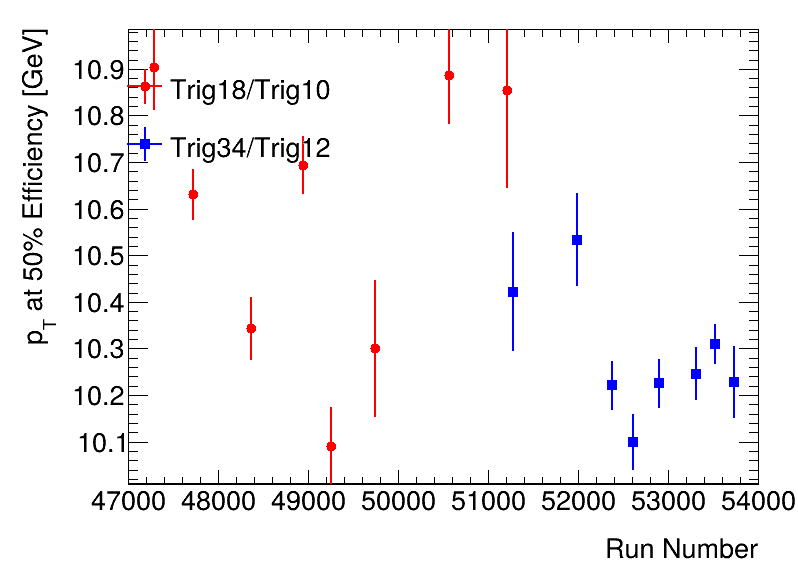
\includegraphics[width=0.48\linewidth]{Figures/trigger_efficiency/50pct_efficiency_vs_run.png}
    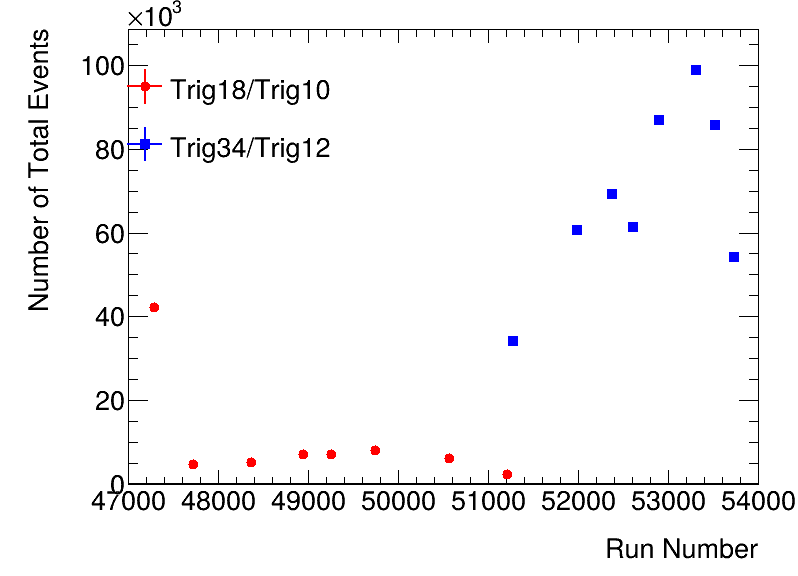
\includegraphics[width=0.48\linewidth]{Figures/trigger_efficiency/total_events_vs_run.png}
    \caption{Run-by-run 50\% efficiency point of the Jet10 trigger (left) and total MB events with a reconstructed jet with $p_T > 7$ GeV (right).}
    \label{fig:runbyrun_50pct}
\end{figure}

To account for these effects, the dataset is divided into three efficiency regimes: early 0~mrad, mid-time 0~mrad, and 1.5~mrad running. 
This approach minimizes biases from changing calibrations and varying trigger statistics.
The resulting run range dependent efficiencies are shown in Figure~\ref{fig:jet10_vs_time_efficiency_comparison}.

\begin{figure}
    \centering
    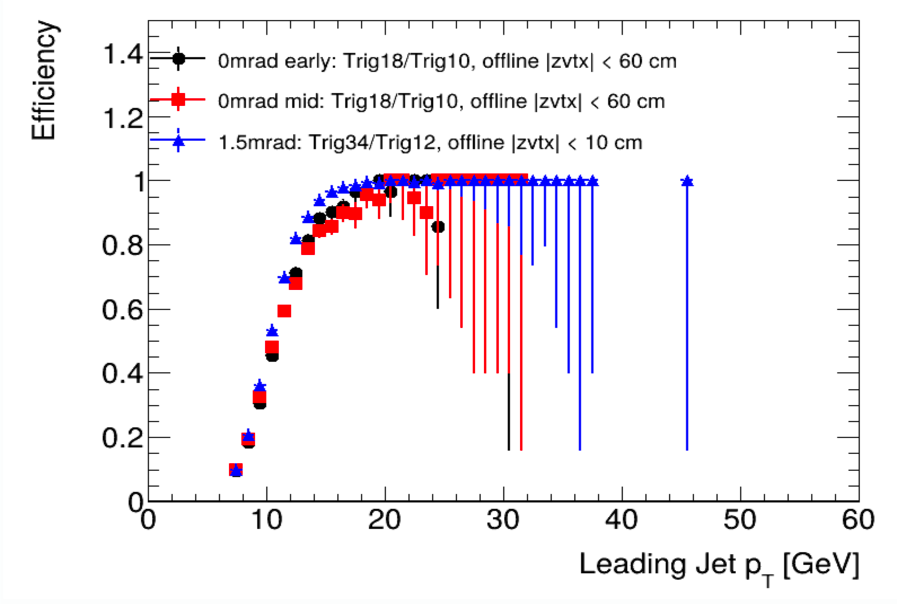
\includegraphics[width=0.7\linewidth]{Figures/trigger_efficiency/jet10_vs_time_efficiency_comparison.png}
    \caption{Jet10 trigger efficiency for three run ranges in the analysis: early 0 mrad (black), mid-time 0 mrad (red) and 1.5 mrad (blue).}
    \label{fig:jet10_vs_time_efficiency_comparison}
\end{figure}

\subsection{Jet Trigger Efficiency Fitting and Systematics}
\label{sec:jet_trigger_eff}

Jet trigger efficiencies are determined using \texttt{TEfficiency}, defined as the ratio of leading jet $p_{T}$ distributions for jet-triggered events to minimum bias events. 
Efficiencies are parameterized using the functional form
\begin{equation}
    \epsilon(p_T) = [0] + [1]/pow(1+exp(-[3]*(p_T-[2])),[4])
\end{equation}
consistent with the approach used in PPG09 and approximating a logistic turn-on behavior with asymptotic behavior at 1 (full efficiency).

Fits are performed using a binomial likelihood. 
Figure~\ref{fig:jet_trig_fitting} shows the resulting efficiency curves as a function of uncalibrated leading jet $p_{T}$. 
Statistical uncertainties are estimated by sampling the fit parameters within their covariance matrix to extract 1$\sigma$ variations. 

\begin{figure}
    \centering
    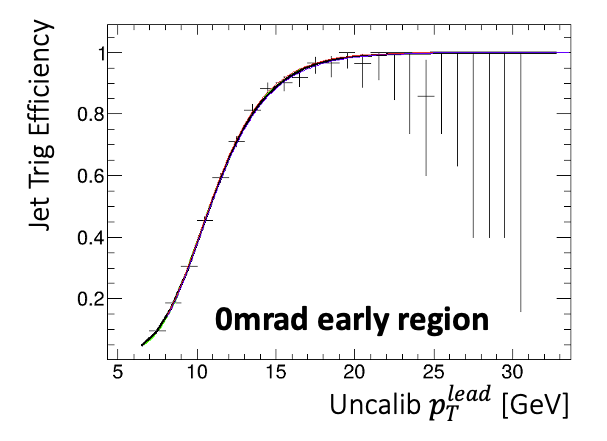
\includegraphics[width=0.48\linewidth]{Figures/trigger_efficiency/jet_trig_eff_fit_0mrad_early.png}
    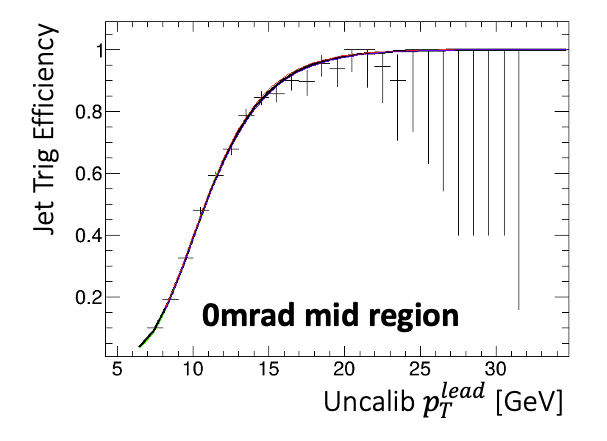
\includegraphics[width=0.48\linewidth]{Figures/trigger_efficiency/jet_trig_eff_fit_0mrad_mid.png}
    
\includegraphics[width=0.48\linewidth]{{Figures/trigger_efficiency/jet_trig_eff_fit_1.5mrad}.png}
    \caption{Jet trigger efficiency curve fitting using data from early 0mrad (top left), mid-time 0mrad (top right) and 1.5mrad (bottom) run ranges. Nominal fit shown in black with fits defined from 1$\sigma$ variations on fit parameters shown in red/blue.}
    \label{fig:jet_trig_fitting}
\end{figure}

\subsection{MBD Vertex Efficiencies}
\label{sec:mbd_vertex_eff}

The MBD vertex efficiency is evaluated in simulation and is studied as a function of jet $p_{T}$ and transverse region $E_{T}$.
Figure~\ref{fig:mbd_eff_meas_range} shows the MBD vertex efficiency both as a function of jet $p_{T}$ and transverse region $E_{T}$ across the PPG10 measurement ranges.

%\begin{figure}
%    \centering
%    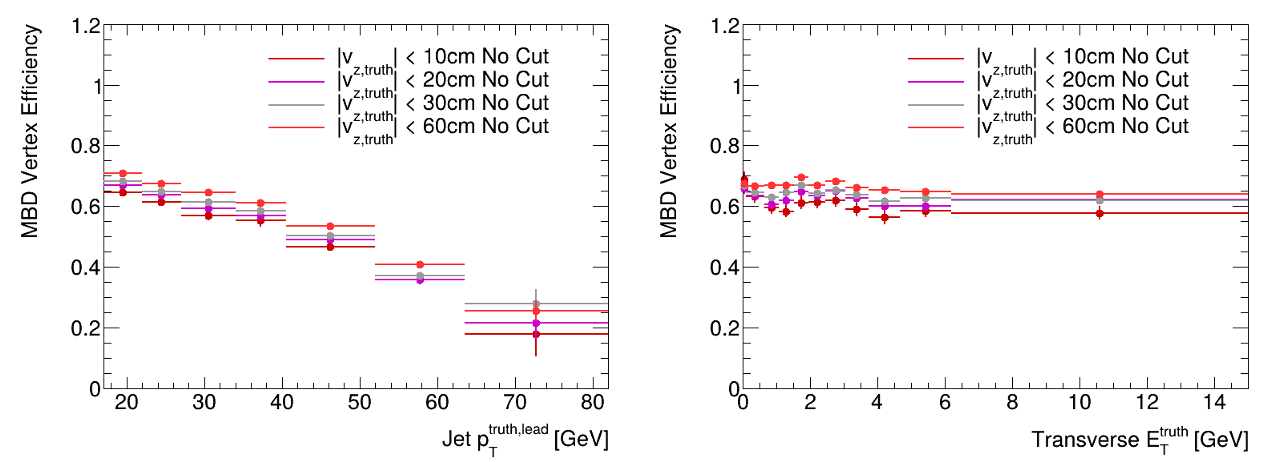
\includegraphics[width=\linewidth]{Figures/mbd_vertex_efficiency/vertex_eff_vs_zvertex_range.png}
%    \caption{MBD vertex efficiency versus leading jet $p_{T}$ (left) and transverse region $E_{T}$ (right) for different $z_{\mathrm{vtx}}$ ranges.}
%    \label{fig:mbd_eff_zvertex_range}
%\end{figure}

\begin{figure}
    \centering
    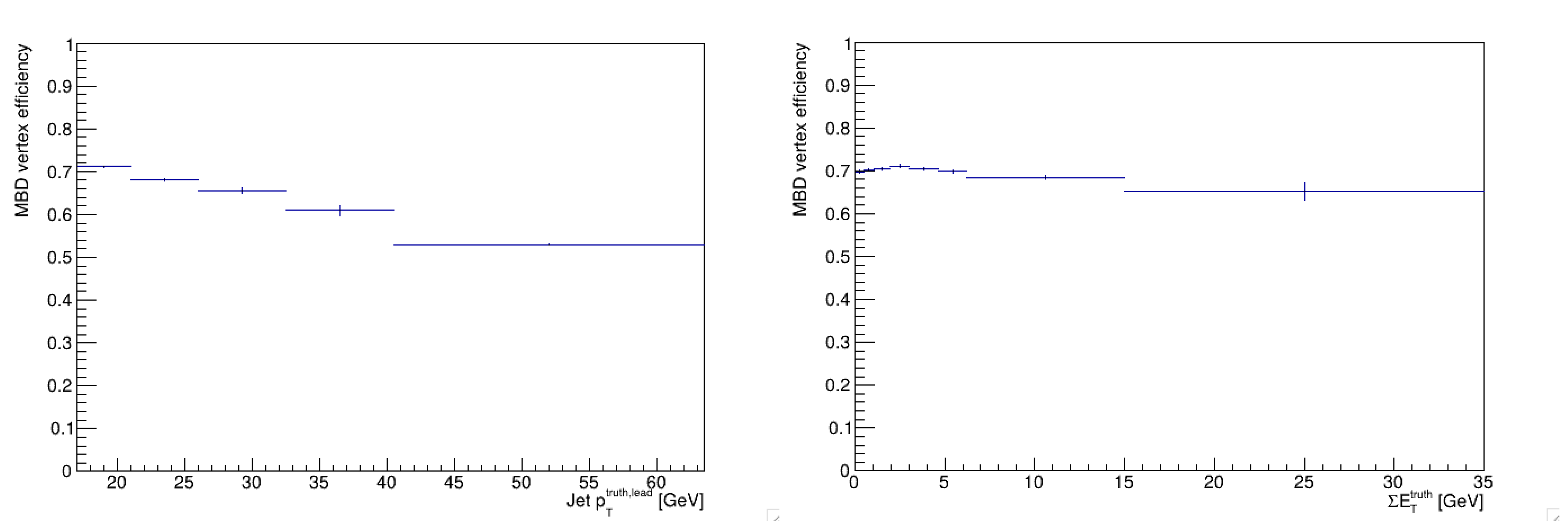
\includegraphics[width=\linewidth]{Figures/mbd_vertex_efficiency/vertex_eff_meas_range.png}
    \caption{MBD vertex efficiency versus leading jet $p_{T}$ (left) and transverse region $E_{T}$ (right) for PPG10 measurement binning.}
    \label{fig:mbd_eff_meas_range}
\end{figure}

The transverse region dependence of the vertex efficiency is shown in Fig.~\ref{fig:mbd_eff_tr}. 
After normalizing out the dominant jet $p_{T}$ dependence, residual variations with transverse region $E_{T}$ are below the 5\% level. 
The vertex efficiency is applied at the truth level after the unfolding procedure and details on this application are provided in Section~\ref{sec:analysis}.

\begin{figure}
    \centering
    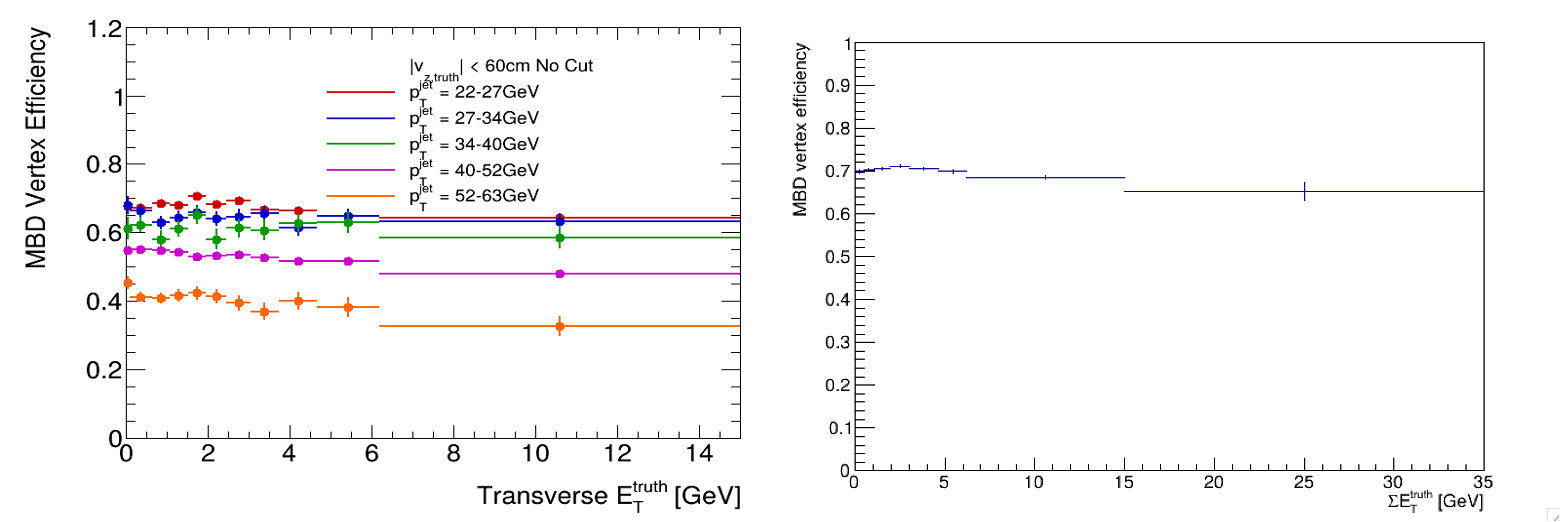
\includegraphics[width=\linewidth]{Figures/mbd_vertex_efficiency/vertex_eff_pt_slices.png}
    \caption{MBD vertex efficiency versus transverse region $E_{T}$ shown for slices in leading jet $p_{T}$.}
    \label{fig:mbd_eff_tr}
\end{figure}
